\documentclass{ximera}

%\usepackage{todonotes}

\newcommand{\todo}{}

\usepackage{tkz-euclide}
\tikzset{>=stealth} %% cool arrow head
\tikzset{shorten <>/.style={ shorten >=#1, shorten <=#1 } } %% allows shorter vectors

\usepackage{tkz-tab}  %% sign charts
\usetikzlibrary{decorations.pathreplacing} 

\usetikzlibrary{backgrounds} %% for boxes around graphs
\usetikzlibrary{shapes,positioning}  %% Clouds and stars
\usetikzlibrary{matrix} %% for matrix
\usepgfplotslibrary{polar} %% for polar plots
\usetkzobj{all}
\usepackage[makeroom]{cancel} %% for strike outs
%\usepackage{mathtools} %% for pretty underbrace % Breaks Ximera
\usepackage{multicol}

\usepackage{polynom}



\usepackage[many]{tcolorbox}  %% for titled boxes
\newtcolorbox{xbox}[1]{%
    tikznode boxed title,
    enhanced,
    arc=0mm,
    interior style={white},
    attach boxed title to top center= {yshift=-\tcboxedtitleheight/2},
    fonttitle=\bfseries,
    colbacktitle=white,coltitle=black,
    boxed title style={size=normal,colframe=white,boxrule=0pt},
    title={#1}}


\usepackage{array}
\setlength{\extrarowheight}{+.1cm}   
\newdimen\digitwidth
\settowidth\digitwidth{9}
\def\divrule#1#2{
\noalign{\moveright#1\digitwidth
\vbox{\hrule width#2\digitwidth}}}





\newcommand{\RR}{\mathbb R}
\newcommand{\R}{\mathbb R}
\newcommand{\N}{\mathbb N}
\newcommand{\Z}{\mathbb Z}

%\renewcommand{\d}{\,d\!}
\renewcommand{\d}{\mathop{}\!d}
\newcommand{\dd}[2][]{\frac{\d #1}{\d #2}}
\newcommand{\pp}[2][]{\frac{\partial #1}{\partial #2}}
\renewcommand{\l}{\ell}
\newcommand{\ddx}{\frac{d}{\d x}}
\newcommand{\ddt}{\frac{d}{\d t}}

\newcommand{\zeroOverZero}{\ensuremath{\boldsymbol{\tfrac{0}{0}}}}
\newcommand{\inftyOverInfty}{\ensuremath{\boldsymbol{\tfrac{\infty}{\infty}}}}
\newcommand{\zeroOverInfty}{\ensuremath{\boldsymbol{\tfrac{0}{\infty}}}}
\newcommand{\zeroTimesInfty}{\ensuremath{\small\boldsymbol{0\cdot \infty}}}
\newcommand{\inftyMinusInfty}{\ensuremath{\small\boldsymbol{\infty - \infty}}}
\newcommand{\oneToInfty}{\ensuremath{\boldsymbol{1^\infty}}}
\newcommand{\zeroToZero}{\ensuremath{\boldsymbol{0^0}}}
\newcommand{\inftyToZero}{\ensuremath{\boldsymbol{\infty^0}}}



\newcommand{\numOverZero}{\ensuremath{\boldsymbol{\tfrac{\#}{0}}}}
\newcommand{\dfn}{\textbf}
%\newcommand{\unit}{\,\mathrm}
\newcommand{\unit}{\mathop{}\!\mathrm}
\newcommand{\eval}[1]{\bigg[ #1 \bigg]}
\newcommand{\seq}[1]{\left( #1 \right)}
\renewcommand{\epsilon}{\varepsilon}
\renewcommand{\iff}{\Leftrightarrow}

\DeclareMathOperator{\arccot}{arccot}
\DeclareMathOperator{\arcsec}{arcsec}
\DeclareMathOperator{\arccsc}{arccsc}
\DeclareMathOperator{\si}{Si}
\DeclareMathOperator{\proj}{proj}
\DeclareMathOperator{\scal}{scal}


\newcommand{\tightoverset}[2]{% for arrow vec
  \mathop{#2}\limits^{\vbox to -.5ex{\kern-0.75ex\hbox{$#1$}\vss}}}
\newcommand{\arrowvec}[1]{\tightoverset{\scriptstyle\rightharpoonup}{#1}}
\renewcommand{\vec}{\mathbf}
\newcommand{\veci}{\vec{i}}
\newcommand{\vecj}{\vec{j}}
\newcommand{\veck}{\vec{k}}
\newcommand{\vecl}{\boldsymbol{\l}}

\newcommand{\dotp}{\bullet}
\newcommand{\cross}{\boldsymbol\times}
\newcommand{\grad}{\boldsymbol\nabla}
\newcommand{\divergence}{\grad\dotp}
\newcommand{\curl}{\grad\cross}
%\DeclareMathOperator{\divergence}{divergence}
%\DeclareMathOperator{\curl}[1]{\grad\cross #1}


\colorlet{textColor}{black} 
\colorlet{background}{white}
\colorlet{penColor}{blue!50!black} % Color of a curve in a plot
\colorlet{penColor2}{red!50!black}% Color of a curve in a plot
\colorlet{penColor3}{red!50!blue} % Color of a curve in a plot
\colorlet{penColor4}{green!50!black} % Color of a curve in a plot
\colorlet{penColor5}{orange!80!black} % Color of a curve in a plot
\colorlet{fill1}{penColor!20} % Color of fill in a plot
\colorlet{fill2}{penColor2!20} % Color of fill in a plot
\colorlet{fillp}{fill1} % Color of positive area
\colorlet{filln}{penColor2!20} % Color of negative area
\colorlet{fill3}{penColor3!20} % Fill
\colorlet{fill4}{penColor4!20} % Fill
\colorlet{fill5}{penColor5!20} % Fill
\colorlet{gridColor}{gray!50} % Color of grid in a plot

\newcommand{\surfaceColor}{violet}
\newcommand{\surfaceColorTwo}{redyellow}
\newcommand{\sliceColor}{greenyellow}




\pgfmathdeclarefunction{gauss}{2}{% gives gaussian
  \pgfmathparse{1/(#2*sqrt(2*pi))*exp(-((x-#1)^2)/(2*#2^2))}%
}


%%%%%%%%%%%%%
%% Vectors
%%%%%%%%%%%%%

%% Simple horiz vectors
\renewcommand{\vector}[1]{\left\langle #1\right\rangle}


%% %% Complex Horiz Vectors with angle brackets
%% \makeatletter
%% \renewcommand{\vector}[2][ , ]{\left\langle%
%%   \def\nextitem{\def\nextitem{#1}}%
%%   \@for \el:=#2\do{\nextitem\el}\right\rangle%
%% }
%% \makeatother

%% %% Vertical Vectors
%% \def\vector#1{\begin{bmatrix}\vecListA#1,,\end{bmatrix}}
%% \def\vecListA#1,{\if,#1,\else #1\cr \expandafter \vecListA \fi}

%%%%%%%%%%%%%
%% End of vectors
%%%%%%%%%%%%%

%\newcommand{\fullwidth}{}
%\newcommand{\normalwidth}{}



%% makes a snazzy t-chart for evaluating functions
%\newenvironment{tchart}{\rowcolors{2}{}{background!90!textColor}\array}{\endarray}

%%This is to help with formatting on future title pages.
\newenvironment{sectionOutcomes}{}{} 



%% Flowchart stuff
%\tikzstyle{startstop} = [rectangle, rounded corners, minimum width=3cm, minimum height=1cm,text centered, draw=black]
%\tikzstyle{question} = [rectangle, minimum width=3cm, minimum height=1cm, text centered, draw=black]
%\tikzstyle{decision} = [trapezium, trapezium left angle=70, trapezium right angle=110, minimum width=3cm, minimum height=1cm, text centered, draw=black]
%\tikzstyle{question} = [rectangle, rounded corners, minimum width=3cm, minimum height=1cm,text centered, draw=black]
%\tikzstyle{process} = [rectangle, minimum width=3cm, minimum height=1cm, text centered, draw=black]
%\tikzstyle{decision} = [trapezium, trapezium left angle=70, trapezium right angle=110, minimum width=3cm, minimum height=1cm, text centered, draw=black]


\outcome{Define accumulation functions.}
\outcome{Calculate and evaluate accumulation functions.}
\outcome{State the First Fundamental Theorem of Calculus.}
\outcome{Take derivatives of accumulation functions using the First Fundamental Theorem of Calculus.}
\outcome{Use accumulation functions to find information about the original function.}
\outcome{Understand the relationship between the function and the derivative of its accumulation function.}

\title[Dig-In:]{The First Fundamental Theorem of Calculus}

\begin{document}
\begin{abstract}
  The rate that accumulated area under a curve grows is described
  identically by that curve.
\end{abstract}
\maketitle

\section{Accumulation functions}


While the definite integral computes a signed area, which is a fixed
number, there is a way to turn it into a function.

\begin{definition}
A given a function $f$, an \dfn{accumulation function} is
\[
F(x) = \int_a^x f(t) \d t.
\]
\end{definition}
One thing that you might notice is that an accumulation function seems
to have two variables: $x$ and $t$. Let's see if we can explain
this. Consider the following graph:
\begin{image}
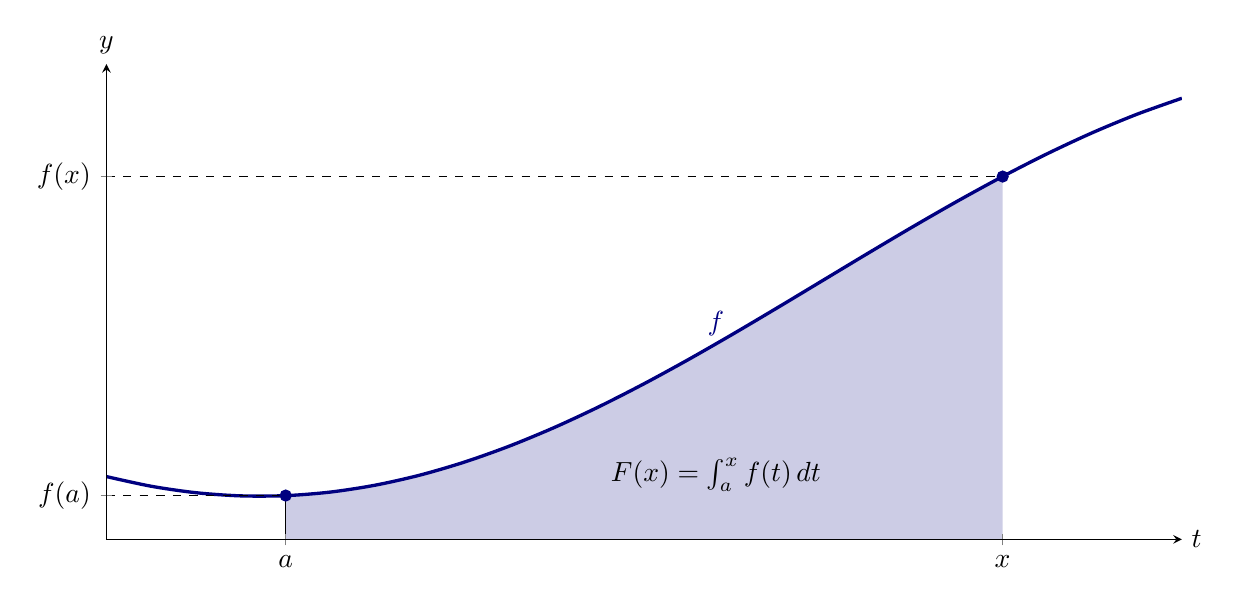
\begin{tikzpicture}
	\begin{axis}[
            domain=0:6, ymax=2.2,xmax=6,
            axis lines =left, xlabel=$t$, ylabel=$y$,
            width=6in,
            height=3in,
            every axis y label/.style={at=(current axis.above origin),anchor=south},
            every axis x label/.style={at=(current axis.right of origin),anchor=west},
            xtick={1,5}, ytick={.203,1.679},
            xticklabels={$a$,$x$}, yticklabels={$f(a)$,$f(x)$},
            axis on top,
          ]
          \addplot [draw=none,fill=fillp,domain=(1:5)] {sin(deg((x - 4)/2)) + 1.2} \closedcycle;
          \addplot [very thick,penColor, smooth,domain=(0:6)] {sin(deg((x - 4)/2)) + 1.2};

          \addplot [textColor,dashed] plot coordinates {(0,1.679) (5,1.679)};
          \addplot [textColor,dashed] plot coordinates {(0,.203) (1,.203)};
          %\addplot [textColor,dashed] plot coordinates {(5,0) (5,1.679)};
          \addplot [textColor] plot coordinates {(1,0) (1,.203)};

          \addplot [color=penColor,fill=penColor,only marks,mark=*] coordinates{(1,.203)};  %% closed hole         
          \addplot [color=penColor,fill=penColor,only marks,mark=*] coordinates{(5,1.679)};  %% closed hole       
          \node at (axis cs:3.4,.3) [textColor] {$F(x) = \int_a^x f(t) \d t$};
          \node at (axis cs:3.4,1) [penColor] {$f$};
        \end{axis}
\end{tikzpicture}
\end{image}

An accumulation function $F$ measures the signed area in the region
$[a,x]$ between $f$ and the $t$-axis. Hence $t$ is playing the role of
a ``place-holder'' that allows us to evaluate $f$. On the other hand,
$x$ is the \textbf{specific number} that we are using to bound the
region that will determine the area between $f$ and the $t$-axis, and
hence the value of $F$.
\begin{question}
  Given
  \[
  F(x) = \int_{-3}^x 4 \d t,
  \]
  what is $F(5)$?
  \begin{prompt}
    \[
    F(5) = \answer{32}
    \]
  \end{prompt}
  \begin{question}
    What is $F(-5)$?
    \begin{prompt}
      \[
      F(-5) = \answer{-8}
      \]
    \end{prompt}
  \end{question}
\end{question}


\begin{example} 
Consider the following accumulation function for $f(x) = x^3$.
\[
F(x) = \int_{-1}^x t^3 \d t.
\]
Considering the interval $[-1,1]$, where is $F$ increasing? Where
is $F$ decreasing? When does $F$ have local extrema?

\begin{explanation}
We can see a graph of $f$ along with the signed area measured by the
accumulation function below
\begin{image}
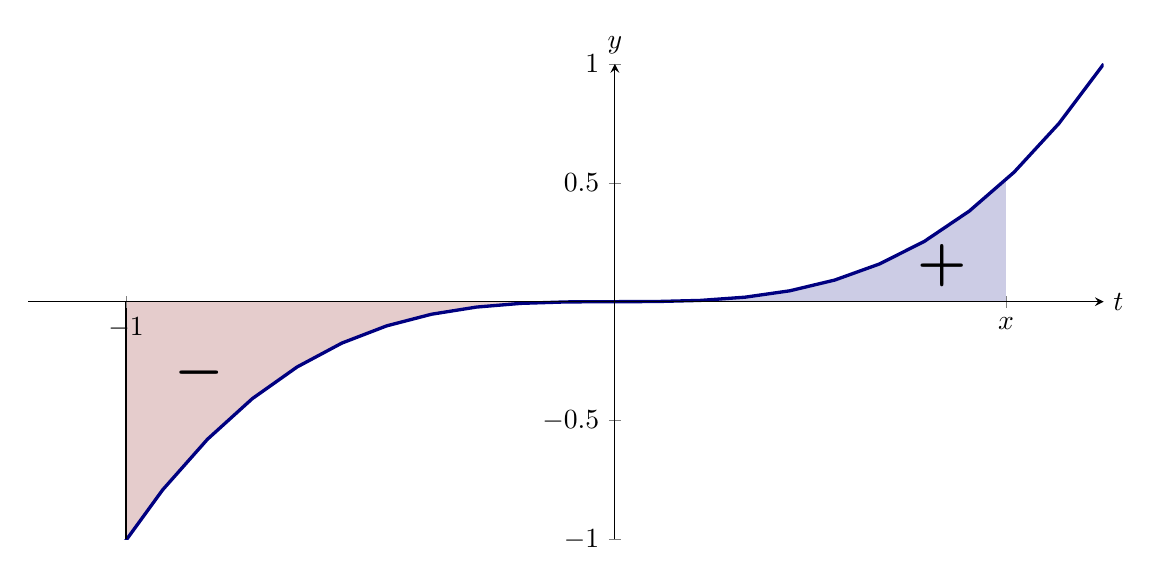
\begin{tikzpicture}
  \begin{axis}[
      xmin=-1.2, xmax=1,ymin=-1,ymax=1,domain=-1:1,
      axis lines =center, xlabel=$t$, ylabel=$y$,
      every axis y label/.style={at=(current axis.above origin),anchor=south},
      every axis x label/.style={at=(current axis.right of origin),anchor=west},
      xtick={-1,.8}, 
      xticklabels={$-1$,$x$}, 
      axis on top,
      width=6in,
      height=3in,
    ] 
    \addplot [draw=none, fill=fillp,domain=0:.8] {x^3} \closedcycle;
    \addplot [draw=none, fill=filln,domain=-1:0] {x^3} \closedcycle;
    \addplot [penColor,very thick,domain=-1.2:1,] {x^3};
    
    \addplot [textColor] plot coordinates {(-1,0) (-1,-1)};

    \node at (axis cs:.67,.15) [textColor] {\scalebox{2}{$\boldsymbol+$}};
    \node at (axis cs:-.85,-.3) [textColor] {\scalebox{2}{$\boldsymbol-$}};
  \end{axis}
\end{tikzpicture}
%\caption{The integral $\int_{-1}^x t^3 \d t$ measures the shaded area.}
%\label{figure:accumulationeg}
\end{image}
The accumulation function starts off at zero, and then as $x$ grows,
$F$ is \wordChoice{\choice{increasing}\choice[correct]{decreasing}} as
the function accumulates negatively signed area.

However when $x>0$, $F$ starts to accumulate positively signed area,
and hence is
\wordChoice{\choice[correct]{increasing}\choice{decreasing}}. Thus $F$
is increasing on $(0,1)$, decreasing on $(-1,0)$ and hence has a local
minimum at $(0,0)$.
\end{explanation}
\end{example}

Working with the accumulation function leads us to a question, what is
\[
\int_a^x f(x) \d x
\]
when $x< a$? The general convention is that 
\[
\int_a^b f(x) \d x = -\int_b^a f(x) \d x. 
\]
With this in mind, let's consider one more example.

\begin{example} 
Consider the following accumulation function for $f(x) = x^3$.
\[
F(x) = \int_{-1}^x t^3 \d t.
\]
Where is $F$ increasing? Where is $F$ decreasing? When does
$F$ have local extrema?
\begin{explanation}
From our previous example, we know that $F$ is increasing on
$(0,1)$. Since $f$ continues to be positive at $t=1$ and beyond, $F$
is \wordChoice{\choice[correct]{increasing}\choice{decreasing}} on
$(0,\infty)$. On the other hand, we know from our previous example
that $F$ is
\wordChoice{\choice{increasing}\choice[correct]{decreasing}} on
$(-1,0)$.
\begin{image}
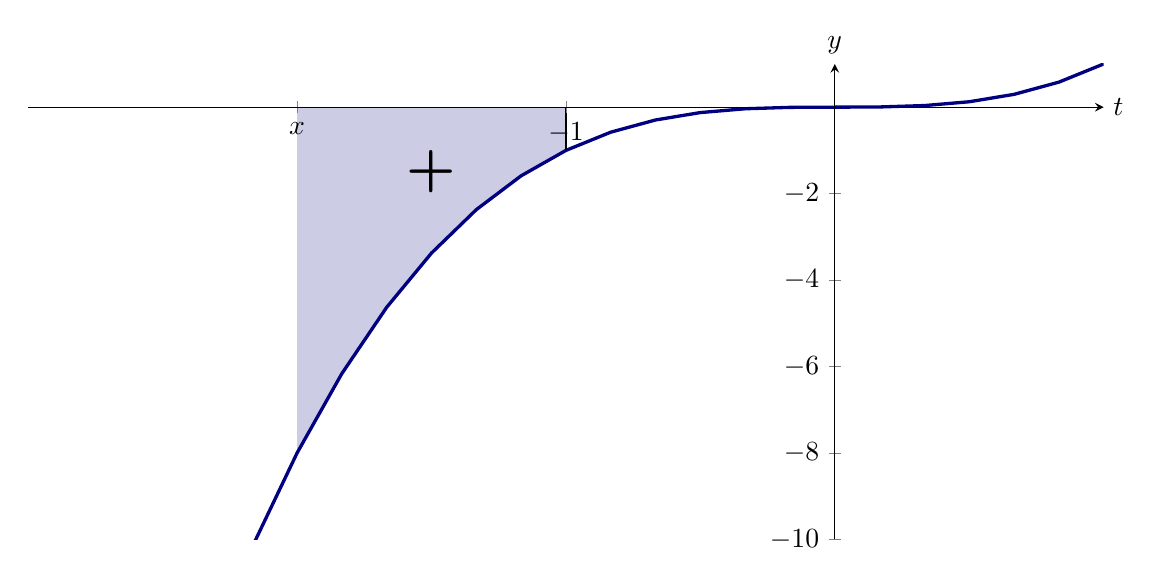
\begin{tikzpicture}
  \begin{axis}[
      xmin=-3, xmax=1,ymin=-10,ymax=1,domain=-3:1,
      axis lines =center, xlabel=$t$, ylabel=$y$,
      every axis y label/.style={at=(current axis.above origin),anchor=south},
      every axis x label/.style={at=(current axis.right of origin),anchor=west},
      xtick={-2,-1}, 
      xticklabels={$x$,$-1$}, 
      axis on top,
      width=6in,
      height=3in,
    ] 
    \addplot [draw=none, fill=fillp,domain=-2:-1] {x^3} \closedcycle;
    \addplot [penColor,very thick] {x^3};

    \addplot [textColor] plot coordinates {(-1,0) (-1,-1)};
    
    \node at (axis cs:-1.5,-1.5) [textColor] {\scalebox{2}{$\boldsymbol+$}};
  \end{axis}
\end{tikzpicture}
%\caption{The integral $\int_{-1}^x t^3 \d t$ measures the shaded
%  area. Note, since $x<-1$, the area has positive sign.}
\end{image}
For values to the left of $t=-1$, $F$ is still decreasing, as less and
less positively signed area is accumulated. Hence $F$ is increasing on
$(0,\infty)$, decreasing on $(-\infty,0)$ and hence has an absolute
minimum at $(0,0)$.
\end{explanation}
\end{example}
The key point to take from these examples is that an accumulation
function
\[
F(x) = \int_a^x f(t) \d t
\]
is increasing precisely when $f$ is positive and is decreasing
precisely when $f$ is negative. In short, it seems that $f$ is
behaving in a similar fashion to $F'$.



\section{The First Fundamental Theorem of Calculus}



Let $f$ be a continuous function on the real numbers and consider
\[
  F(x) = \int_a^x f(t)\d t.
\]
From our previous work we know that $F$ is increasing when $f$ is
positive and $F$ is decreasing when $f$ is negative. Moreover, with
careful observation, we can even see that $F$ is concave up when $f'$
is positive and that $F$ is concave down when $f'$ is negative.
Thinking about what we have learned about the relationship of a
function to its first and second derivatives, it is not too hard to
guess that there must be a connection between $F'$ and the function
$f$. This is a good guess, check out our next theorem:


\begin{theorem}[First Fundamental Theorem of Calculus]\index{First Fundamental Theorem of Calculus}
Suppose that $f$ is continuous on the real numbers and let
\[
  F(x)=\int_a^x f(t)\d t.
\]
Then $F'(x)=f(x)$.
\end{theorem}
The First Fundamental Theorem of Calculus says that an accumulation
function of $f$ is an antiderivative of $f$. Another way of saying
this is:
\begin{image}
  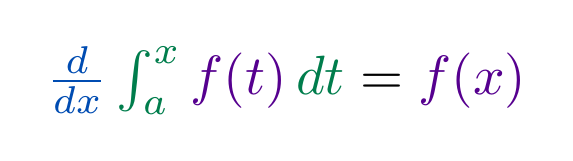
\begin{tikzpicture}[scale=2,every node/.style={transform shape}]
    \node at (0,0) {
      $\color{blue!70!green}\ddx \color{green!70!black!70!blue}\int_a^x\color{purple!50!blue!90!black}f(t)\color{green!70!black!70!blue}\d t\color{black} = \color{purple!50!blue!90!black}f(x)$
      };
  \end{tikzpicture}
\end{image}
This could be read as:%%BADBAD I want this all in bold and with colors
\begin{quote}\large\textbf{The \textcolor{blue!70!green}{rate} that \textcolor{green!70!black!70!blue}{accumulated area} under a  \textcolor{purple!50!blue!90!black}{curve} grows is described identically by that  \color{purple!50!blue!90!black}{curve}.}
\end{quote}

Now that we are working with accumulation functions, let's see what
happens when we compose them with other functions.

\begin{example}
  Find the derivative of
  \[
  F(x) = \int_2^{x^2} \ln t \d t.
  \]
  \begin{explanation}
    Consider 
    \[
    G(x) = \int_2^x \ln t \d t
    \]
    and set $h(x) = \answer[given]{x^2}$. Now
    \[
    F(x) = G(h(x)).
    \]
    The First Fundamental Theorem of Calculus states that $G'(x) = \ln
    x$. The chain rule gives us
    \begin{align*}
      F'(x) &= G'(h(x)) h'(x) \\
      &= \ln (h(x)) h'(x) \\
      &= \answer[given]{\ln (x^2) 2x}.
    \end{align*}
  \end{explanation}
\end{example}

Let's practice this a bit more.

\begin{example}
  Find the
  derivative of
  \[
  F(x) = \int_{\cos x}^5 t^3\d t.
  \]
  \begin{explanation}
    Consider
    \[
    G(x) = - \int_5^x t^3 \d t
    \]
    and set $h(x) = \answer[given]{\cos(x)}$. Now
    \[
    F(x) = G(h(x)).
    \]
    The First Fundamental Theorem of Calculus states that $G'(x) = -x^3$. The chain rule gives us
    \begin{align*}
      F'(x) &= G'(h(x))h'(x)\\
      &=-h(x)^3 h'(x)\\
      &=\answer[given]{-\cos^3(x) (-\sin(x))}.
    \end{align*}
  \end{explanation}
\end{example}

\begin {example}
Given the graph of a function $f$ on the interval $[-1,5]$, sketch the graph of the accumulation function 
 \[
F(x) = \int_{-1}^x f(t) \d t, \hspace{0.2in}   -1\le x\le 5.
\]
\begin{image}
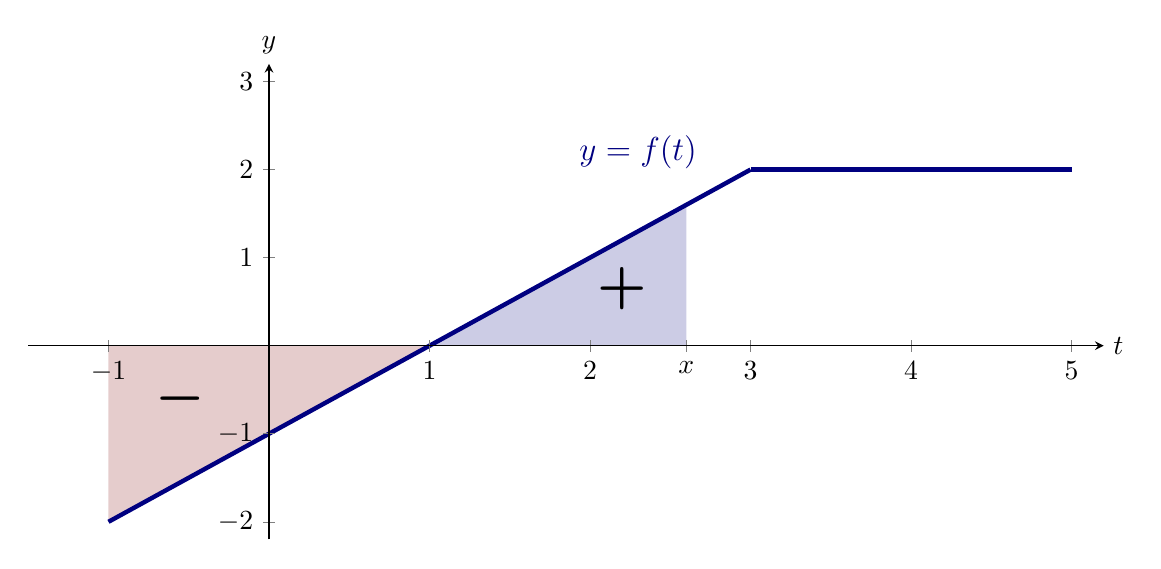
\begin{tikzpicture}
  \begin{axis}[
      xmin=-1.5, xmax=5.2,ymin=-2.2,ymax=3.2,domain=-1:5.5,
      axis lines =center, xlabel=$t$, ylabel=$y$,
      every axis y label/.style={at=(current axis.above origin),anchor=south},
      every axis x label/.style={at=(current axis.right of origin),anchor=west},
      xtick={-1,0,1,2,2.6,3,4,5}, 
      xticklabels={$-1$,$0$,$1$,$2$,$x$,$3$,$4$,$5$}, 
      axis on top,
      width=6in,
      height=3in,
    ] 
    \addplot [draw=none, fill=fillp,domain=1:2.6] {x-1 } \closedcycle;
    \addplot [draw=none, fill=filln,domain=-1:1] {x-1} \closedcycle;
    \addplot [penColor,ultra thick,domain=-1:3] {x-1 };
      \addplot [penColor,ultra thick,domain=3:5] {2 };
   
    \node at (axis cs:2.2,.65) [textColor] {\scalebox{2}{$\boldsymbol+$}};
    \node at (axis cs:-.55,-.6) [textColor] {\scalebox{2}{$\boldsymbol-$}};
      \node at (axis cs:2.3,2.2) [penColor] {\large$y=f(t)$};
  \end{axis}
\end{tikzpicture}
%\caption{The integral $\int_{-1}^x t^3 \d t$ measures the shaded area.}
%\label{figure:accumulationeg}
\end{image}
\begin{explanation}
First, we evaluate $F$ at some significant points.
\[
F(-1) = \int_{-1}^{-1} f(t) \d t=\answer[given]{0}.
\]
\[
F(0) = \int_{-1}^{0} f(t) \d t=\answer[given]{-1.5}.
\]
\[
F(1) = \int_{-1}^{1} f(t) \d t=\answer[given]{-2}.
\]
\[
F(3) = \int_{-1}^{3} f(t) \d t=\answer[given]{0}.
\]
\[
F(4) = \int_{-1}^{4} f(t) \d t=\answer[given]{2}.
\]
\[
F(5) = \int_{-1}^{5} f(t) \d t=\answer[given]{4}.
\]

Since $F'(x)=f(x)$, it follows that the function $F$ is increasing on the interval
\[
\left(\answer[given]{1},\answer[given]{5}\right)
\]
and decreasing on the interval
\[
\left(\answer[given]{-1},\answer[given]{1}\right).
\]
Since the function $f$, the derivative of $F$, is increasing on $(1,3)$,  $F$ is concave up on the interval
\[
\left(\answer[given]{1},\answer[given]{3}\right).
\]
Since $f$ is constant on the interval  $[3,5]$, $F$ is linear on $[3,5]$. 

The function $F$ has  a local and global minimum at
\[
x=\answer[given]{1},
\]
and the global maximum at
\[
x=\answer[given]{5}.
\]
Now we are ready to sketch the graph of $F$, on the same set of axes as the graph of $f$.
\begin{image}
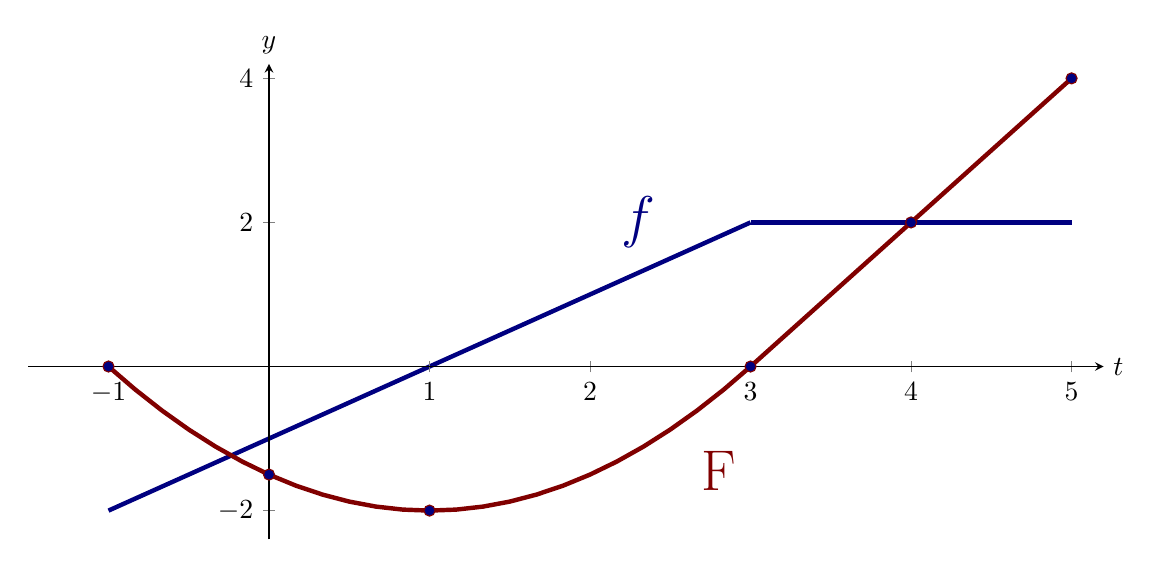
\begin{tikzpicture}
  \begin{axis}[
      xmin=-1.5, xmax=5.2,ymin=-2.4,ymax=4.2,domain=-1:5.5,
      axis lines =center, xlabel=$t$, ylabel=$y$,
      every axis y label/.style={at=(current axis.above origin),anchor=south},
      every axis x label/.style={at=(current axis.right of origin),anchor=west},
      xtick={-1,0,1,2,3,4,5}, 
      xticklabels={$-1$,$0$,$1$,$2$,$3$,$4$,$5$}, 
      axis on top,
      width=6in,
      height=3in,
    ] 
 
    \addplot [penColor,ultra thick,domain=-1:3] {x-1 };
      \addplot [penColor,ultra thick,domain=3:5] {2 };
     \addplot[color=penColor2,fill=penColor,only marks,mark=*] coordinates{(-1,0)};  %% closed hole
        \addplot[color=penColor2,fill=penColor,only marks,mark=*] coordinates{(0,-1.5)};  %% closed hole
      \addplot[color=penColor2,fill=penColor,only marks,mark=*] coordinates{(1,-2)};  %% closed hole
  
      \addplot[color=penColor2,fill=penColor,only marks,mark=*] coordinates{(3,0)};  %% closed hole
        \addplot[color=penColor2,fill=penColor,only marks,mark=*] coordinates{(4,2)};  %% closed hole
      \addplot[color=penColor2,fill=penColor,only marks,mark=*] coordinates{(5,4)};  %% closed hole
      \addplot [penColor2,ultra thick,domain=-1:3] {(1/2)*x^2-x-3/2 };
      \addplot [penColor2,ultra thick,domain=3:5] {2*x-6};
      \node at (axis cs:2.3,2) [penColor] {\huge$f$};
         \node at (axis cs:2.8,-1.45) [penColor2] {\huge F };
  \end{axis}
\end{tikzpicture}
%\caption{The integral $\int_{-1}^x t^3 \d t$ measures the shaded area.}
%\label{figure:accumulationeg}
\end{image}
\end{explanation}
\end{example}

What if $f$ is the velocity function for an object moving along a straight line, i.e. $f(t)=v(t)$, $a\le t\le b$?

What is the meaning of an accumulation function in that case?


We use different variables in that case, since we want $F$ to be a function of time, $t$. With this adjustment, we define the accumulation function $F$ as follows.
\[
  F(t)=\int_a^t v(z)\d z.
\]
Since the integral
\[
 \int_a^t v(z)\d z
\]
gives the displacement of the object on the time interval $[a,t]$, it follows that
\[
s(t)-s(a)= \int_a^t v(z)\d z,
\]
where $s(t)$ gives the position of the object at the time $t$.
If we differentiate this equation with respect to $t$, we get that
\[
s'(t)=\dd t \int_a^t v(z)\d z.
\]
Since $s'(t)=v(t)$, we have that
\[
v(t)=\dd t \int_a^t v(z)\d z.
\]
This is the the First Fundamental Theorem of Calculus!

\end{document}
